\documentclass{article}
\usepackage{amsmath}
\usepackage{geometry}
\geometry{a4paper, margin=1in}
\usepackage{tikz}
\usetikzlibrary{arrows.meta}

\title{Code Explanation: Phytoplankton Strain Dynamics}
\author{}
\date{}

\begin{document}

\maketitle

% ... (Other sections of your LaTeX document)

\subsection{Why is 2*delta instead of delta inside the loop?}

The $2\delta$ inside the loop (for $j = 1$ to $M_s - 1$) and the $\delta$ at the boundaries ($j=0$ and $j=M_s$) in the strain update equation are due to how we model the probabilistic shift of biomass between neighboring strains. Let's illustrate with an example:

Imagine we have 5 strains ($M_s = 4$), each represented by a circle:

\begin{figure}[h]
    \centering
    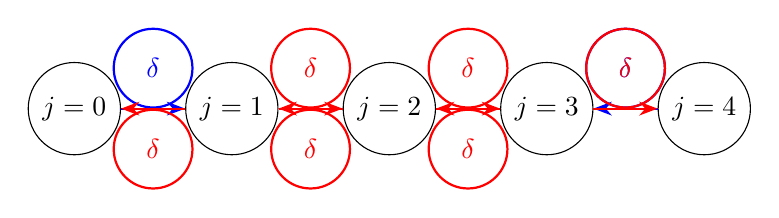
\begin{tikzpicture}[
        every node/.style={circle, draw, minimum size=1cm},
        arrow/.style={-Stealth, thick},
        delta/.style={blue, arrow},
        twodelta/.style={red, arrow}
      ]
        \node (s0) at (0,0) {$j=0$};
        \node (s1) at (2,0) {$j=1$};
        \node (s2) at (4,0) {$j=2$};
        \node (s3) at (6,0) {$j=3$};
        \node (s4) at (8,0) {$j=4$};

        % Arrows for delta (boundaries)
        \draw[delta] (s0) -- (s1) node[midway, above] {$\delta$};
        \draw[delta] (s4) -- (s3) node[midway, above] {$\delta$};

        % Arrows for 2*delta (inner strains)
        \draw[twodelta] (s1) -- (s0) node[midway, below] {$\delta$};
        \draw[twodelta] (s1) -- (s2) node[midway, above] {$\delta$};
        \draw[twodelta] (s2) -- (s1) node[midway, below] {$\delta$};
        \draw[twodelta] (s2) -- (s3) node[midway, above] {$\delta$};
        \draw[twodelta] (s3) -- (s2) node[midway, below] {$\delta$};
        \draw[twodelta] (s3) -- (s4) node[midway, above] {$\delta$};


    \end{tikzpicture}
    \caption{Biomass transfer between strains. Blue arrows (boundaries): transfer probability $\delta$. Red arrows (inner strains): $\delta$ to each neighbor, totaling $2\delta$ transfer from each inner node.}
    \label{fig:strain_transfer_example}
\end{figure}

Let $\delta = 0.2$ represent the probability that biomass shifts from one strain to a neighboring strain.

* \textbf{Strain 0 ($j=0$):}  This strain is at the boundary.  It can only lose biomass to strain 1. The fraction of biomass that remains in strain 0 is $(1 - \delta) = (1 - 0.2) = 0.8$.

* \textbf{Strain 1 ($j=1$):} This strain is in the interior. It can lose biomass to *both* strain 0 and strain 2.  It loses a fraction $\delta$ to strain 0 and a fraction $\delta$ to strain 2.  The total fraction of biomass lost by strain 1 is $2\delta = 2 \times 0.2 = 0.4$.  Therefore, the fraction of biomass that *remains* in strain 1 is $(1 - 2\delta) = (1 - 0.4) = 0.6$.

* \textbf{Strain 2 ($j=2$):}  Similar to strain 1, it loses $\delta$ to strain 1 and $\delta$ to strain 3, for a total loss of $2\delta$. The remaining fraction is $(1 - 2\delta)$.

* \textbf{Strain 4 ($j=4$):} This strain is also at a boundary. It only loses biomass to strain 3. The remaining fraction is $(1 - \delta)$.

This explains why the update equation uses $(1 - \delta)$ for the boundary strains and $(1 - 2\delta)$ for the inner strains. The $2\delta$ accounts for the biomass transferred to *both* neighboring strains.

% ... (Rest of your LaTeX document)
\subsection{Why only one delta at the ends and two deltas in the beginning? (Question and Answer)}

\textbf{Question:} Why is the biomass transfer probability $\delta$ used for the boundary strains ($j=0$ and $j=M_s$) while $2\delta$ is used for the inner strains ($j=1$ to $M_s-1$) in the update equation?  It seems like there are "more deltas in the beginning."

\textbf{Answer:} The difference between $2\delta$ inside the loop and $\delta$ at the boundaries is not about "more deltas at the beginning" but about the *number of neighbors* each strain has.

\begin{itemize}
    \item \textbf{Inner Strains ($j = 1$ to $M_s - 1$):} Each inner strain has *two* neighbors. When biomass shifts, each inner strain loses some biomass to *both* of these neighbors. If the probability of shifting to *one* neighbor is $\delta$, then the total probability of shifting biomass *away* from an inner strain is $2\delta$. That's why the update equation for inner strains uses $(1 - 2\delta)$: it represents the fraction of biomass that *remains* in the strain after transfers to *both* neighbors.

    \item \textbf{Boundary Strains ($j = 0$ and $j = M_s$):} The strains at the boundaries only have *one* neighbor. Strain $j=0$ only has a neighbor to its right (strain $j=1$), and strain $j=M_s$ only has a neighbor to its left (strain $j=M_s-1$). They can't transfer biomass "outside" the array. Therefore, they only lose biomass to *one* neighbor. The fraction of biomass lost is just $\delta$. The update equation uses $(1 - \delta)$ because only one transfer is possible.
\end{itemize}

\textbf{Analogy:} Imagine a row of people. Each person represents a strain. They're throwing balls (representing biomass) to their neighbors.

\begin{itemize}
    \item \textbf{People in the middle:} Each person in the middle throws balls to *both* the person on their left and the person on their right. They lose a total of 2 balls (if each throw has a probability of 1).
    \item \textbf{People at the ends:} The people at the ends only have *one* neighbor. They can only throw a ball to that one neighbor. They lose only 1 ball.
\end{itemize}

\textbf{In summary:} The difference between $2\delta$ inside the loop and $\delta$ at the boundaries is not about "more deltas at the beginning" but about the *number of neighbors* each strain has. Inner strains have two neighbors, so they lose biomass to both, leading to a total loss probability of $2\delta$. Boundary strains have only one neighbor, so they lose biomass to only that one neighbor, leading to a loss probability of $\delta$. This difference is essential for correctly modeling the biomass transfer at the edges of the system.
\end{document}
